\chapterimage{slike/Mavrica.jpg} % Chapter heading image

\chapter{Koherenca}

V tem poglavju bomo spoznali \index{Koherenca}koherenco. To je lastnost
valovanja, ki je tesno povezana s pojavom interference. Ohlapno pravimo,
da je koherentno tisto valovanje, s katerim se posrečijo interferenčni
poskusi\index{Interferenca}.  

\section{Youngov poskus}

\index{Interferenca}Interferenčnih pojavov ni mogoče opazovati z
vsakim svetlobnim izvorom. Da bi to razumeli, si oglejmo interferenco
valovanja, ki vpada na dve ozki reži (tako imenovani \index{Youngov poskus}Youngov 
poskus\footnote{Angleški znanstvenik Thomas Young, 1773--1829.}). 
Navadno predpostavimo, da
sta obe reži osvetljeni z istim ravnim valom. Delni valovanji, ki
izhajata iz rež, imata tako ves čas poskusa enako polarizacijo, enako
frekvenco in enako fazo. Ker sta dolžini poti delnih valovanj od reže do dane 
točke na zaslonu različni, nastane na oddaljenem
zaslonu interferenčni vzorec (slika~\ref{fig:Young}). Vendar se  
interferenca pojavi le v primeru,
ko je faza valovanja, ki vpada na reži, konstantna. Svetloba s konstantno
fazo nastane na primer v kvalitetnih laserjih in zanjo pravimo, da je koherentna.
Svetloba iz navadnih svetil ima spremenljivo fazo in zato ne da
interferenčnega vzorca. Zanjo pravimo, da ni koherentna. 
\begin{figure}[h]
\centering
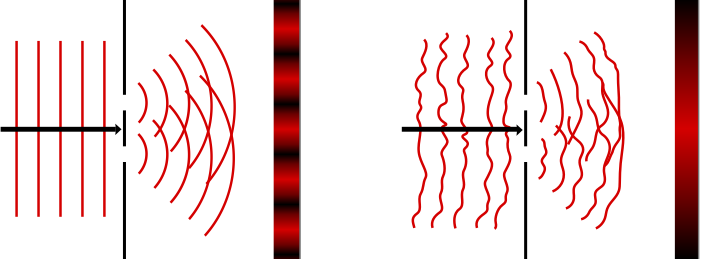
\includegraphics[width=10truecm]{slike/02_Young.pdf}
\caption{Youngov poskus na dveh režah. Le če je vpadno valovanje koherentno, 
se pojavi na zaslonu interferenčni vzorec (levo). Nekoherentno valovanje s spremenljivo
fazo ne da interferenčnega vzorca (desno).}
\label{fig:Young}
\end{figure}

\vglue-5truemm
Svetloba navadnih svetil, na primer plinskih razelektritvenih cevi, 
je zaradi vrste nastanka kaotične narave. 
Atomi v njih sevajo neodvisno, zato se faza izsevanega valovanja neprestano
spreminja. Približno konstantna je le znotraj nekega karakterističnega
časa. Če je pri interferenčnem poskusu karakteristični čas spreminjanja
faze krajši od zakasnitve med valovanjema zaradi različno
dolgih poti, pride na danem mestu zaslona izmenično do konstruktivne in 
destruktivne interference. Čas spreminjanja je praviloma
bistveno krajši od časa opazovanja, zato utripanja ne vidimo in 
zaznamo povprečno razmazano sliko. Interferenčni poskus se ne 
posreči zaradi majhne časovne koherence\index{Koherenca!časovna},
karakterističnemu času spreminjanja faze pa rečemo 
\index{Koherenčni čas}koherenčni čas
$t_{c}$. Časovno koherenco bomo natančneje obravnavali v razdelku
(\ref{sec:casovna-koherenca}), zaenkrat povejmo le, da je časovna
koherenca vezana na fazno razliko med točkami, ki ležijo
vzdolž smeri širjenja valovanja. 

Poleg časovne koherence na interferenčno sliko pomembno vpliva tudi
\index{Koherenca!prostorska}prostorska koherenca, ki je posledica
končne dimenzije svetila. Svetloba, ki na reži vpada iz različnih delov
svetila, ima namreč različno fazo zaradi razlike v dolžini poti 
do rež. Ta faza se prišteje fazni razliki zaradi različno dolgih poti 
od rež do zaslona, zato se interferenčne proge na zaslonu nekoliko 
premaknejo. Če je fazna razlika žarkov iz različnih
delov svetila večja od fazne razlike za režami, se celotna interferenčna
slika na zaslonu izpovpreči. Interferenca se pri Youngovem poskusu
pojavi, kadar sta reži razmaknjeni le toliko, da je povprečna fazna
razlika manjša od $2\pi$. Največjemu prečnemu razmiku, ki še da interferenco,
rečemo prečna koherenčna razdalja\index{Koherenčna razdalja} $d_{c}$. 
Prostorska koherenca, ki jo bomo podrobneje spoznali v razdelku 
(\ref{Prostorska-koherenca}),
je torej vezana na fazno razliko med točkami, ki ležijo prečno 
na smer širjenja valovanja.

Poudarimo še enkrat, da je pojem koherence statističen.
Če je koherenčni čas $t_{c}$ dolg v primerjavi s časom opazovanja,
se seštevajo amplitude valovanj in pojavi se interferenčna slika.
Ta se slučajno spreminja z značilnim časom $t_{c}$. Če pa so razlike
poti večje od $ct_{c}$ ali razmik rež večji od $d_{c}$, gledamo
le povprečno sliko in interferenčne proge izginejo.

\section{Koherenca navadnih svetil}
\label{chap:kns}
Obravnavajmo plinsko razelektritveno cev in z
ustreznim filtrom izberimo eno samo spektralno črto. Ta črta naj ima
osrednjo frekvenco $\nu_{0}$ in končno frekvenčno širino $\Delta\nu$.
Privzamemo, da je glavni prispevek k razširitvi spektralne črte posledica
medatomskih trkov.

Celotna izsevana svetloba je vsota delnih valov, ki izhajajo iz posameznih
atomov in so med seboj neodvisni. Vsak delni val ohranja konstantno fazo
med dvema trkoma, to je v intervalu dolžine $t_{c}$. Valovni paket dolžine 
$t_{c}$ tako vsebuje frekvence v pasu $\Delta \nu$,
za katerega velja $t_{c}\Delta\nu\sim1$. Koherenčni čas je torej
kar reda velikosti obratne vrednosti spektralne širine svetlobe. Povsem
monokromatsko valovanje bi imelo neskončen koherenčni čas in bi bilo
popolnoma koherentno.

Zapišimo še izsevano polje takega svetila. 
Jakost električnega polja v izbrani točki prostora je vsota delnih
valov, ki izvirajo iz raznih delov izvora. Vsak atom v izvoru, naj
jih bo $N$, seva neodvisno, zato so tudi delna valovanja med seboj
neodvisna. Posamična valovanja ohranjajo konstantno fazo v času med
dvema trkoma atoma $t_{c}$. Zaradi enostavnosti privzamemo,
da so amplitude $E_{1}$ in polarizacije izsevanih polj posameznih atomov enake. 
Električno poljsko jakost $E$ v izbrani točki prostora potem 
zapišemo kot vsoto posameznih prispevkov
\begin{equation}
E=E_{1}\sum_{n=1}^{N}e^{i\phi_{n}(t)},
\label{eq:amplituda-random}
\end{equation}
kjer se faza polja $\phi_{n}(t)$, ki ga izseva posamezni atom, naključno
spremeni ob trku z drugim atomom. Povprečje vsote polj je nič, 
povprečni kvadrat skupnega polja, ki je sorazmeren
z gostoto svetlobnega toka, pa je $NE_{1}^{2}$. Zaradi slučajnosti faz je 
slučajna tudi faza celotnega polja in se gotovo povsem spremeni v času, ko se
spremeni faza posameznih prispevkov, to je $t_{c}$. S tako svetlobo bomo videli 
interferenco na režah, če bo razlika poti delnih valovanj manjša od $c\, t_{c}$.

Oglejmo si izračun
na primeru. Imejmo $N=100$ neodvisnih atomov, ki se jim faza naključno
spreminja s karakterističnim časom $t_{c}=10/\nu$, kjer je $\nu$
frekvenca valovanja. Na sliki (\ref{fig:amplituda-intenziteta}) sta
prikazana časovna poteka amplitude $E$ (enačba \ref{eq:amplituda-random})
in $|E|^{2}$.
\begin{figure}
\centering
\def\svgwidth{140truemm} 
\input{slike/02_fluktuacije02.pdf_tex}\\
\def\svgwidth{140truemm} 
\input{slike/02_fluktuacije01.pdf_tex}\\
\def\svgwidth{140truemm} 
\input{slike/02_fluktuacije03.pdf_tex}\\
\def\svgwidth{140truemm} 
\input{slike/02_fluktuacije04.pdf_tex}\\
\caption{Zgoraj: shematski prikaz jakosti električnega polja 
ravnega vala s konstantno fazo (rdeča črta) in jakosti električnega
polja navadnega svetila (modra črta) kot funkcije časa. 
Spodaj: pripadajoča vrednost $|E|^2$ v primeru ravnega vala (rdeča črta) in 
v primeru svetlobe iz navadnega svetila (modra črta) kot funkcija
časa. Modra črtkana črta je povprečna vrednost
$\frac{1}{T}\int_{-T/2}^{T/2}E(t+t')E^{*}(t+t')dt'$
s časom integracije $T=t_{c}$.}
\label{fig:amplituda-intenziteta}
\end{figure}
Za primerjavo je prikazan tudi ravni val\index{Ravni val} $E=\sqrt{N}E_{1}e^{-i\omega t}$
s konstantno fazo in pripadajoč $|E|^{2}$, ki je sorazmeren z gostoto svetlobnega
toka. Ta je v primeru ravnega vala konstantna, medtem ko je povprečna gostota
svetlobnega toka iz navadnega svetila približno konstantna le znotraj $t_{c}$.

\section{Časovna koherenca}
\label{sec:casovna-koherenca}

Časovno koherenco\index{Koherenca!časovna} je najpreprosteje obravnavati 
z \index{Michelsonov interferometer}Michelsonovim 
interferometrom\footnote{Ameriški fizik in nobelovec Albert Abraham Michelson, 1852--1931.},
ki je prikazan na sliki (\ref{fig:michelson}). 
\begin{figure}[!h]
\centering
\def\svgwidth{85truemm} 
\input{slike/02_Michelson.pdf_tex}\\
\caption{\label{fig:michelson}Michelsonov interferometer. Svetlobo
iz izvora $P$ usmerimo skozi kolimacijsko lečo (L) na polprepustno
zrcalo (PZ), s čimer jo razdelimo na dva snopa. S premikanjem 
enega od zrcal (Z) spreminjamo zakasnitev enega delnega snopa in
na detektorju izmenično zaznavamo oslabitve in ojačitve -- opazujemo interferenco.}
\end{figure}

Valovanje iz točke $P$ na polprepustnem zrcalu razdelimo na dva delna snopa, 
nato enega s premikanjem zrcala zakasnimo za $\tau=2x/c$. Dokler je zakasnitev
$\tau$ manjša od koherenčnega časa $t_{c}$, snopa med seboj interferirata.
Ob premikanju zrcala se na detektorju izmenično pojavljajo ojačitve in 
oslabitve. Pri zakasnitvah, ki so večje od koherenčnega časa, ni stalne fazne 
povezave in na detektorju zaznavamo svetlobo, katere intenziteta ni odvisna od lege
zrcala $x$.

\begin{remark}
S kolimacijsko lečo dosežemo, da je čim več žarkov, ki izhajajo iz
$P$, vzporednih z osjo interferometra. V eksperimentih snop svetlobe 
ni nikoli povsem vzporeden in dolžine poti posameznih žarkov se med
seboj malo razlikujejo. Na detektorju tako za $\tau < t_c$ nastanejo jasno 
vidni interferenčni krogi. Pri večjih vrednostih $\tau$  se kontrast interferenčnih
prog zmanjšuje in pri zakasnitvah, ki so daljše od koherenčnega časa, se 
slika povsem zabriše. 
\end{remark}

Zapišimo ugotovitev še matematično.
Gostota svetlobnega toka na detektorju je sorazmerna s kvadratom jakosti električnega
polja obeh delnih valovanj
\begin{equation}
|E_{d}(t)|^{2}=|E(t)+E(t+\tau)|^{2}=|E(t)|^{2}+|E(t+\tau)|^{2}+2\Re \left(E(t)E^{*}(t+\tau)\right).
\label{eq:Michelson-intenziteta}
\end{equation}
Zakasnitev $\tau$ je določena s premikom pomičnega zrcala $\tau=2x/c$.
Navadno opazujemo v času $T$, ki je dolg v primerjavi s koherenčnim
časom svetlobe, zato izraz povprečimo po času
\begin{eqnarray}
\langle|E_{d}(t)|^{2}\rangle & = & \frac{1}{T}\int_{-T/2}^{T/2}|E{}_{d}(t)|^{2}\, dt\nonumber \\
 & = & 2\langle|E(t)|^{2}\rangle+2\Re\langle E(t)E^{*}(t+\tau)\rangle = 2\langle|E(t)|^{2}\rangle+2\Re G(\tau).
 \label{eq:caskohav}
\end{eqnarray}
Prvi člen je vsota povprečnih prispevkov obeh delnih snopov. Privzeli smo, 
da je povprečje polja neodvisno od izbire časovnega intervala.
Drugi člen opisuje interferenco\index{Interferenca}. 
Za opis smo vpeljali
časovno avtokorelacijsko funkcijo\index{Avtokorelacijska funkcija}
jakosti električnega polja 
\boxeq{eq:avtokorelacija}{
G(\tau)=\frac{1}{T}\int_{-T/2}^{T/2}E(t)E^{*}(t+\tau)\, dt.
}
Za zakasnitve $\tau$, ki so krajše od koherenčnega časa $t_c$, je avtokorelacijska
funkcija različna od nič in na
detektorju zaznamo interferenco. Pri zakasnitvah, ki so precej
daljše od koherenčnega časa $t_{c}$, sta polji $E(t)$ in $E(t+\tau)$
statistično neodvisni in povprečje produkta je enako produktu povprečij.
Ker je $\langle E(t)\rangle=0$, pri velikih zakasnitvah $\tau$ interferenčni
člen izgine.

Priročno je vpeljati normirano avtokorelacijsko funkcijo 
\begin{equation}
g(\tau)=\frac{G(\tau)}{G(0)}.
\label{eq:avtokorelacija-norm}
\end{equation}
Za povsem koherentno valovanje je $|g(\tau)|=1$, za povsem nekoherentno
valovanje je $|g(\tau)|=0,$ za delno koherentna  pa $0<|g(\tau)|<1$.
Praviloma se vrednost $|g(\tau)|$ z naraščajočim $\tau$ zmanjšuje,
saj postaja valovanje za velike časovne zamike vedno manj korelirano.
Ohlapno povedano je koherenčni čas zakasnitev, pri kateri postane
vrednost avtokorelacijske funkcije majhna.
Koherenčni čas\index{Koherenčni čas} $t_{c}$ bolj natančno definiramo 
z normirano avtokorelacijsko funkcijo
\boxeq{eq:koherencni-cas}{
t_{c}=\int_{-\infty}^{\infty}\left|g(\tau)\right|^{2}\, d\tau.
}
Zakasnitev delnih valov je pogosto posledica
različno dolgih optičnih poti, zato namesto koherenčnega časa $t_c$
pogosto uporabljamo koherenčno dolžino\index{Koherenčna dolžina} $l_{c}=c\,t_{c}$. 

\begin{definition}
Pokaži, da v navedenih avtokorelacijskih
funkcijah $g(\tau)$ spremenljivka $t_{c}$ ustreza koherenčnemu času,
kot je definiran v enačbi (\ref{eq:koherencni-cas}), in izračunaj $|g(t_{c})|$ za oba primera.
\begin{equation}
g(\tau)=\begin{cases}
\exp\big(i\omega_{0}\tau-\left|\tau\right|/t_{c}\big),\\
\exp\big(i\omega_{0}\tau-\pi\tau^{2}/2t_{c}^{2}\big),
\end{cases}
\label{eq:gauss-eksponent}
\end{equation}

Ob nalogi (\ref{naloga-spekter}) in v razdelku~(\ref{Razsiritev}) 
bomo spoznali, da sta to avtokorelacijski
funkciji za svetlobo z \index{Spekter!Lorentzov}Lorentzovim spektrom
(razširitev spektralne črte zaradi medatomskih trkov) in Gaussovim spektrom\index{Spekter!Gaussov}
(Dopplerjeva razširitev)\index{Dopplerjeva razširitev}.
\end{definition}

Poglejmo nekaj značilnih vrednosti koherenčnih dolžin. 
Koherenčna dolžina svetlobe, izsevane iz črnega telesa, je $l_{c}=c\,t_{c}\approx 
\hbar c/k_{B}T$ (glej nalogo~\ref{naloga-Planck})\index{Sevanje črnega telesa}. 
Svetloba s Sonca ($T \approx 6000$~K)
ima tako koherenčno dolžino zgolj $\sim 0,4~\si{\micro\metre}$, kar ustreza
koherenčnemu času $t_c \sim 1~\si{fs}$. Svetloba,
izsevana iz LED sijalk\index{LED}, ima koherenčno dolžino $\sim20$--$100~\si{\micro\metre}$.
Živosrebrna svetilka ima za izbrano spektralno črto koherenčno dolžino
do okoli $50~\si{\centi\metre}$, kar ustreza koherenčnemu času $t_c \sim 1,6~\si{ns}$.
Koherenčna dolžina svetlobe, izsevane iz laserjev, je tipično okoli $100~\si{\metre}$, 
v nekaterih vlakenskih laserjih\index{Laser!vlakenski} pa koherenčna dolžina 
presega $100~\si{\kilo\metre}$.

\section{Zveza med avtokorelacijsko funkcijo in spektrom}

Obravnavajmo zdaj koherenco poljubnega valovanja, ki
je v povprečju stacionarno. To pomeni, da se povprečna gostota svetlobnega
toka v času zajemanja, ki traja čas $T$, ne spreminja in da je avtokorelacijska funkcija
odvisna le od $\tau$. Vzorec valovanja razvijemo
v Fourierevo vrsto
\begin{equation}
E(t)=\sum_{n}A_{n}(\omega)e^{-i n \Delta\omega t},\mbox{\hskip1cm}\Delta\omega=\frac{2\pi}{T}.
\end{equation}
Amplitude $A_{n}(\omega)$ so slučajne spremenljivke, ki predstavljajo delež polja pri 
krožni frekvenci $\omega=n\Delta\omega$, čas opazovanja $T$ pa naj bo bistveno daljši od $t_{c}$. 
Potem zapišemo amplitude $A_n$
\begin{equation}
A_{n}(\omega)=\frac{1}{T}\int_{-T/2}^{T/2}E(t)\, e^{i\omega t}\, dt.\label{eq:amplituda-An}
\end{equation}
Kvadrat $|A_{n}(\omega)|^{2}$ je sorazmeren z gostoto svetlobnega toka pri krožni
frekvenci $\omega$ in predstavlja intenziteto\index{Intenziteta}
valovanja\footnote{Intenziteto valovanja na splošno vpeljemo kot $I = |E|^2$, gostota svetlobnega
toka pa je $j = \varepsilon \varepsilon_0 c |E|^2/2$ z enotami W/m$^2$ (enačba~\ref{eq:jcw}). 
Kadar predfaktorji niso pomembni, pogosto uporabljamo krajši izraz.}. 
Intenziteto svetlobe pri $\omega$, deljeno z intervalom $\Delta\omega$, imenujemo  
\index{Spekter}spekter $S(\omega)$
\begin{equation}
S(\omega)=\frac{|A_{n}(\omega)|^{2}}{\Delta\omega}=\frac{T}{2\pi}|A_{n}(\omega)|^{2}.
\end{equation}
Vstavimo še amplitudo $A_{n}$ (enačba \ref{eq:amplituda-An}) in dobimo 
\begin{equation}
S(\omega) =\frac{1}{2\pi T}\int\int_{-T/2}^{T/2}E(t)E^{*}(t^{\prime})\, 
e^{-i\omega(t^{\prime}-t)}\, dt\, dt^{\prime}.
\end{equation}
Uvedemo novo spremenljivko $\tau=t^{\prime}-t$ in zapišemo
\begin{equation}
S(\omega)=\frac{1}{2\pi T}\int_{-\infty}^{\infty}e^{-i\omega\tau}d\tau\int_{-T/2}^{T/2}E(t)E^{*}(t+\tau)\, dt.
\label{eq:spekter}
\end{equation}
Integral po $t$ je ravno enak korelacijski funkciji $G(\tau)$ 
(enačba~\ref{eq:avtokorelacija}). Privzeli smo, da velja $T\gg t_{c}$, zato 
je korelacijska funkcija na mejah integracije po $\tau$ praktično enaka nič in 
meje integracije smo lahko raztegnili do neskončnosti. Zveza, ki smo jo dobili, je 
\index{Wiener-Hinčinov izrek} 
Wiener-Hinčinov izrek\footnote{Ameriški matematik Norbert Wiener, 1894--1964, in 
ruski matematik Aleksander Jakovljevič Hinčin, 1894--1959.}
\boxeq{eq:spekter-zveza}{
S(\omega)=\frac{1}{2\pi}\int_{-\infty}^{\infty}G(\tau)e^{-i\omega\tau}\, 
d\tau\;\Longleftrightarrow\; G(\tau)=\int_{-\infty}^{\infty}S(\omega)e^{i\omega\tau}\, 
d\omega.
}
Spekter v povprečju stacionarne svetlobe je torej Fouriereva transformiranka 
avtokorelacijske funkcije svetlobnega polja. 

Vendar je spekter, ki smo ga zapisali z enačbo~(\ref{eq:spekter}), zapisan za izbran 
vzorec valovanja, ki traja čas $T$, in je tudi slučajna spremenljivka. Če je proces
nestacionaren, moramo izrek preoblikovati, tako da namesto količin $S$ in $G$ zapišemo
povprečne količine. Povprečni spekter dobimo tako, da naredimo
limito $T \rightarrow \infty$. 
\begin{equation}
\langle S (\omega) \rangle = \lim_{T\to \infty}S(\omega).
\end{equation}
Za povprečni spekter velja, da je enak Fourierevi transformiranki 
povprečne avtokorelacijske funkcije svetlobnega polja.

Iz Wiener-Hinčinovega izreka (enačba~\ref{eq:spekter-zveza}) neposredno sledi, da je 
koherenca nekega valovanja tesno povezana z njegovim spektrom in 
koherenčni čas $t_{c}$ povezan s spektralno 
širino svetlobe $\gamma$. Velja (glej nalogo~\ref{naloga:gammatc})\index{Koherenčni čas}
\boxeq{eq:spektralna-sirina-zveza}{
\gamma=\frac{1}{t_{c}}.
}
Valovanje z dolgim $t_c$ ima zelo majhno spektralno širino (ozek spekter), 
valovanje s kratkim $t_c$ pa ima širok spekter. To je v skladu s primeri, navedenimi na koncu
prejšnjega razdelka: svetloba s Sonca ima širok spekter in zelo kratek koherenčni čas, 
svetloba iz laserjev pa ima praviloma ozko spektralno črto in dolg koherenčni čas. Ugotovimo 
tudi, da lahko valovanju z ustreznim spektralnim filtriranjem podaljšamo koherenčni čas.
\begin{definition}
\label{naloga:gammatc}
Formalno vpeljemo spektralno širino kot 
\begin{equation}
\gamma=\frac{1}{2\pi\int_{-\infty}^{\infty}\left|s(\omega)\right|^{2}\, d\omega}; \quad
\mathrm{kjer~je} \quad
s(\omega)=\frac{S(\omega)}{\int_{-\infty}^{\infty}S(\omega) d\omega} =\frac{S(\omega)}{G(0)}
\label{eq:spektralna-sirina}
\end{equation}
normirani spekter. 
Z uporabo enačbe za koherenčni čas $t_{c}$ (enačba \ref{eq:koherencni-cas})
pokaži, da je spektralna širina obratno sorazmerna s koherenčnim
časom (enačba \ref{eq:spektralna-sirina-zveza}) ne glede na
obliko spektra. \\
Namig: Uporabi Parsevalov izrek, ki pravi:
\begin{equation}
\int_{-\infty}^{\infty}\left|f(t)\right|^{2}\, dt={2\pi}
\int_{-\infty}^{\infty}\left|F(\omega)\right|^{2}\, d\omega,
\end{equation}
kjer je 
\beq
F(\omega)=\frac{1}{2\pi} \int_{-\infty}^{\infty}f(t)e^{-i\omega\tau}\, d\tau
\eeq
Fouriereva transformiranka funkcije $f(t)$.
\end{definition}

Za zgled Wiener-Hinčinovega izreka vzemimo primer, ki je predstavljen na 
sliki~(\ref{fig:amplituda-intenziteta}). 
Ker so trki med atomi naključni, je avtokorelacijska funkcija eksponentno pojemajoča
\beq
g(\tau)=e^{i\omega_{0}\tau} e^{-\tau/t_{c}}.
\label{eq:g-primer}
\eeq
Vemo, da je spekter take svetlobe Lorentzove 
oblike\index{Spekter!Lorentzov} (glej nalogo~\ref{naloga-spekter})
\begin{equation}
s(\omega)=\frac{1}{\pi}\frac{\gamma}{(\omega-\omega_{0})^{2}+\gamma^{2}},
\label{eq:spekter-primer}
\end{equation}
pri čemer je $\gamma=1/t_{c}$ spektralna širina. 
Normirani spekter $s(\omega)$ in ustrezna avtokorelacijska funkcija $g(\tau)$ 
sta prikazana na sliki~(\ref{fig:SpekterAc}). 
Točke na grafih 
predstavljajo spekter in izračunano avtokorelacijsko funkcijo 
za integracijski čas $T=100\,t_{c}$. Za primerjavo sta z rdečo 
krivuljo prikazana tudi pričakovani spekter (enačba~\ref{eq:spekter-primer}) in avtokorelacijska
funkcija (enačba~\ref{eq:g-primer}). Zaradi končnega
časa $T$ pri izračunu povprečja se spekter iz simulacije nekoliko razlikuje
od pričakovanega. 
\begin{figure}[h]
\centering
\def\svgwidth{65truemm} 
\input{slike/02_spekter.pdf_tex}\qquad
\def\svgwidth{65truemm} 
\input{slike/02_avtokorelacija.pdf_tex}
\caption{Spekter in avtokorelacijska funkcija valovanja s slike~(\ref{fig:amplituda-intenziteta})}
\label{fig:SpekterAc}
\end{figure}

\begin{definition}
\label{naloga-spekter}
Imejmo dve vrsti svetlobe. Prva naj ima avtokorelacijsko funkcijo, ki je eksponentno pojemajoča, druga
pa ima avtokorelacijsko funkcijo Gaussove oblike (enačbi~\ref{eq:gauss-eksponent}). Pokaži, da sta njuna
spektra oblike\index{Spekter!Gaussov}\index{Spekter!Lorentzov}
\begin{equation}
s(\omega)=
\frac{1}{\pi}\frac{\gamma}{(\omega-\omega_{0})^{2}+\gamma^{2}} \quad \mathrm{in} \quad 
s(\omega)= \frac{1}{\sqrt{2}\pi\gamma}\exp\big(-
\frac{\left(\omega-\omega_{0}\right)^{2}}{2\pi\gamma^{2}}\big),
\end{equation}
kjer je $\gamma=1/t_{c}$ spektralna širina. 
\end{definition}

Spektralne črte atomov so pogosto Lorentzove oblike, kar je posledica
eksponentnega razpada stanj (naravna širina). Dodatno se spektralne
črte razširijo zaradi trkov med atomi, vendar tudi to vodi do približno Lorentzove
oblike spektra. V plinih je pogosto prevladujoča razširitev črt
zaradi Dopplerjevega pojava (glej razdelek~\ref{Razsiritev}). Spekter 
Dopplerjevo razširjene svetlobe je Gaussove oblike in iz enačbe~(\ref{eq:spekter-zveza})
sledi, da je v tem primeru tudi avtokorelacijska funkcija Gaussove oblike.
\vglue1truecm

\begin{definition}\label{naloga-Planck}
Numerično pokaži, da je koherenčni čas svetlobe, ki jo oddaja črno telo s 
temperaturo $T$, približno enak $t_{c}\approx{\hbar}/{k_{B}T}$.\index{Sevanje črnega telesa}
Normirani spekter sevanja črnega telesa zapišemo 
kot \index{Spekter!Planckov}Planckov spekter 
\begin{equation}
s(\omega)=\frac{15}{\pi^{4}} \frac{\hbar^4\omega^3}{(kT)^4}/\left(e^{\hbar\omega/kT}-1\right)
\quad \textrm{za}~\omega >0,~\textrm{sicer}~s(\omega) = 0.
\label{eq:Planckov-spekter}
\end{equation}
\end{definition}

\begin{remark}\index{Fouriereva spektroskopija}
V prejšnjem razdelku smo spoznali, da časovno avtokorelacijsko funkcijo
merimo z Michelsonovim interferometrom. Dobljena povezava med merjeno
avtokorelacijo in izračunanim spektrom je osnova za Fourierevo 
spektroskopijo,
pri kateri določimo absorpcijski ali emisijski spekter
snovi iz izmerjene avtokorelacijske funkcije. Tak pristop
ima nekatere pomembne prednosti pred drugimi metodami in se danes
precej uporablja, posebej v infrardečem delu EM valovanja (tako imenovana
metoda FTIR - {\it Fourier-transform infrared spectroscopy}).\index{Infrardeče valovanje}\index{FTIR}
\end{remark}

\section{Prostorska koherenca}
\label{Prostorska-koherenca}
\index{Koherenca!prostorska}
Vrnimo se k Youngovemu poskusu\index{Youngov poskus} in interferenci
\index{Interferenca} na dveh ozkih režah. Osvetljujmo zdaj zaslon, v katerem sta dve odprtini,
s svetilom končnih razsežnosti. Svetilo naj sveti skoraj enobarvno
svetlobo in naj bo na simetrali med odprtinama, kot kaže slika~(\ref{fig:shema-interferenca}).

Žarka, ki izhajata iz sredine svetila (polna rdeča črta), 
opravita do odprtin v ravnini A enako dolgo pot in povzročita na zaslonu B 
interferenčne proge. Žarka, ki izhajata z roba izvora (prekinjena rdeča črta), 
imata do odprtin različno dolgo pot, zato nastane med njima fazna razlika že do ravnine A, 
ki se prišteje fazni razliki do ravnine B. Interferenčne proge, ki jih tvorita 
robna žarka, so premaknjene glede na proge sredinskih žarkov. Ker so žarki z roba
statistično neodvisni od žarkov iz sredine, z njimi
ne interferirajo. Celotni interferenčni vzorec je zato kar vsota interferenčnih
vzorcev žarkov iz različnih delov svetila. Če je razlika poti za žarke
iz različnih delov velikosti valovne dolžine $\lambda$, se celotna
interferenčna slika na zaslonu B izpovpreči.

\begin{figure}[h]
\centering
\def\svgwidth{140truemm} 
\input{slike/02_precnaKoherenca.pdf_tex}
\caption{Shema interferenčnega eksperimenta z razsežnim svetilom}
\label{fig:shema-interferenca}
\end{figure}

Razdaljo med odprtinama, pri kateri interferenčne proge
izginejo, imenujemo\index{Koherenčna razdalja} prečna koherenčna razdalja $d_c$. 
Zanjo velja približno 
\begin{equation}
\delta s = d_c\sin\varphi\approx d_c\frac{R}{z}\sim\lambda\;\Rightarrow\;
d_{c}\sim\frac{z\lambda}{R}.
\label{eq:prost_koh}
\end{equation}
\begin{remark}
Pogosto je v uporabi
pojem \index{Koherenčna ploskev}koherenčna ploskev, to je območje, 
v katerem je fazna razlika v povprečju konstantna. Velikost te ploskve je približno $d_{c}^{2}$.
V območju koherenčne ploskve so tudi valovne fronte približno gladke.
Vsekakor moramo paziti, da koherenčne razdalje $d_c$ ne zamenjamo
s koherenčno dolžino $l_c$, ki smo jo vpeljali pri časovni koherenci valovanja. 
\end{remark}

Zapišimo gornje ugotovitve nekoliko bolj natančno. Na zaslonu $B$
izmerimo povprečno gostoto svetlobnega toka, ki je sorazmerna povprečju kvadrata
jakosti električnega polja. To je sestavljeno iz valovanj iz obeh odprtin
\begin{align}
\langle|E|^{2}\rangle & =\langle|K_{1}E_{1}+K_{2}E_{2}|^{2}\rangle\nonumber \\
&=  |K_{1}|^{2}\langle|E_{1}|^{2}\rangle+|K_{2}|^{2}\langle|E_{2}|^{2}\rangle+
2\Re \left( K_{1}K_{2}^{*}\langle E_{1}(t)E_{2}^{*}(t+\tau)\rangle\right).
\end{align}
Pri tem je $\tau=d\sin\vartheta/c$ zakasnitev valovanja iz druge odprtine
glede na valovanje iz prve, faktorja $K_{1}$ in $K_{2}$ pa sta določena
z uklonom na posameznih odprtinah. Interferenčna slika je vsebovana v podobnem 
členu kot pri Michelsonovem interferometru (enačba~\ref{eq:caskohav}), 
le da nastopa v tem primeru namesto avtokorelacijske funkcije
navzkrižna korelacijska funkcija polj $E_{1}$ in $E_{2}$ iz obeh 
odprtin.\index{Navzkrižna korelacijska funkcija} 

Kako je interferenčni člen povezan z lastnostmi svetila, brez težav
doženemo v izbranem primeru skoraj enobarvne svetlobe z osrednjo krožno frekvenco
$\omega$. Tedaj lahko za zakasnitve $\tau$, ki so krajše
od koherenčnega časa, zapišemo 
\begin{equation}
E_{2}(\tau)=E_{2}(0)\, e^{-i\omega\tau}
\end{equation}
 in 
\begin{equation}
\langle E_{1}(t)E_{2}^{*}(t+\tau)\rangle=
\langle E_{1}(t)E_{2}^{*}(t)\rangle 
e^{i\omega\tau}=J(P_{1},P_{2})\, e^{i\omega\tau}.
\end{equation}
Faktor $\Re e^{i\omega\tau}= \cos(\omega \tau) = \cos(kd\sin\vartheta)$ da interferenčne
proge za koherentno osvetlitev zaslona, povprečje produkta polj
v odprtinah ob istem času $J(P_{1},P_{2})=\langle E(P_{1},t)E^{*}(P_{2},t)\rangle$
pa meri stopnjo prečne koherence med obema odprtinama. Od velikosti
tega člena je odvisen kontrast interferenčnih prog. Izračunajmo ga.

Polje v posamezni odprtini je vsota prispevkov iz celega izvora.
\begin{equation}
E(P_{j})=-\frac{i}{\lambda}\int E(\xi,\eta)\frac{e^{iks_{j}}}{s_{j}}\, d\xi\, d\eta.
\end{equation}
Pri tem je $s_{j}$ razdalja med točko na izvoru s koordinato $(\xi,\eta)$  in točko
$P_{j}(x_{j},y_{j})$ v odprtini na ravnini A (glej sliko \ref{fig:shema-interferenca}).
Faktor pred integralom $-i/\lambda$ izhaja iz uklonske teorije (enačba~\ref{eq:Fresnel-Kirchoffov-integral}).
Tako je 
\begin{equation}
J(P_{1},P_{2})=\frac{1}{\lambda^{2}}\int\int\langle E(\xi,\eta)E^{*}(\xi^{\prime},\eta^{\prime})\rangle\frac{e^{ik(s_{1}-s_{2}^{\prime})}}{s_{1}s_{2}^{\prime}}\, d\xi\, d\eta\, d\xi^{\prime}d\eta^{\prime}.\label{eq:field-correlation}
\end{equation}
V izbranem svetilu sevajo atomi neodvisno. Valovanji iz dveh točk svetila,
ki sta razmaknjeni za več kot $\lambda$, sta neodvisni in povprečje
njunega produkta je enako nič. Tako približno velja 
\begin{equation}
\langle E(\xi,\eta)E^{*}(\xi^{\prime},\eta^{\prime})\rangle=\frac{\lambda^{2}}{\pi} \cdot \delta(\xi-\xi^{\prime},\eta-\eta^{\prime})\langle|E(\xi,\eta)|^{2}\rangle.
\label{eq:delta-Zernike}
\end{equation}
Faktor $\lambda^{2}/\pi$ poskrbi za ustrezno normalizacijo. 
Naj bo oddaljenost svetila od zaslona $A$
veliko večja od dimenzije svetila ($z\gg R$), tako da lahko imenovalec pod integralom
v izrazu~(\ref{eq:field-correlation}) nadomestimo z $z^{2}$ in postavimo
pred integral. Sledi
\begin{equation}
J(P_{1},P_{2})=\frac{1}{\pi z^{2}}\int\langle|E(\xi,\eta)|^{2}\rangle e^{ik(s_{1}-s_{2})}\, d\xi\, d\eta.\label{eq:Zernike1}
\end{equation}
Izraz lahko še nekoliko poenostavimo, če razvijemo $s_{1}$
in $s_{2}$ 
\begin{equation}
s_{j}=\sqrt{z^{2}+(x_{j}-\xi)^{2}+(y_{j}-\eta)^{2}}\approx z+\frac{(x_{j}-\xi)^{2}+(y_{j}-\eta)^{2}}{2z}.
\end{equation}
Pišemo še $\langle|E(\xi,\eta)|^{2}\rangle=I(\xi,\eta)$ ter $x_{2}-x_{1}=\Delta x$
in $y_{2}-y_{1}=\Delta y$. S tem dobimo tako imenovani \index{van Cittert-Zernikov izrek}
van Cittert-Zernikov izrek\footnote{Nizozemski fizik Pieter Hendrik van Cittert, 1889--1959, in 
nizozemski fizik in nobelovec Frits Zernike, 1888--1966.}
\boxeq{eq:Zernike2}{
J(\Delta x,\Delta y)=\frac{e^{-i\phi}}{\pi z^{2}}\int I(\xi,\eta)e^{ik(\Delta 
x\xi+\Delta y\eta)/z}\, d\xi\, d\eta.
}

Faza 
\begin{equation}
\phi=\frac{\pi}{\lambda z}[(x_{2}^{2}+y_{2}^{2})-(x_{1}^{2}+y_{1}^{2})]
\end{equation}
meri skupni premik interferenčnih prog, do katerega pride, kadar svetilo
ne leži na isti osi kot odprtini v zaslonu. Kadar ležita odprtini v ravnini $A$ 
simetrično glede na os svetila, je faza $\phi$ enaka nič.

Dobljeni rezultat si je vredno nekoliko ogledati. Prečno prostorsko
korelacijsko funkcijo $J(P_{1},P_{2})$, ki določa kontrast interferenčnih
prog na zaslonu, smo izrazili kot 2-D  Fourierevo transformiranko intenzitete svetlobe
na samem svetilu (enačba \ref{eq:Zernike2}). 
\begin{remark}
Ob tem se spomnimo,
da velja podobna zveza med jakostjo električnega polja v osvetljeni odprtini 
in njeno Fraunhoferjevo uklonsko sliko (enačba~\ref{eq:FraunhoferApprox}), 
pri čemer so količine, ki nastopajo v obeh zvezah,
povsem različne. Različna je tudi veljavnost obeh izrazov: medtem ko je Fraunhoferjeva
uklonska formula veljavna le v veliki oddaljenosti, za opis uklonske slike v bližnjem polju
pa je treba uporabiti Fresnelov izraz (enačba~\ref{eq:FresnelApprox}), 
je rezultat za $J(P_{1},P_{2})$ (enačba~\ref{eq:Zernike2}) veljaven v obeh območjih.\index{Fraunhoferjev uklon}
\index{Fresnelov uklon}
\end{remark}

Pri velikih razdaljah med točkama $P_{1}$ in $P_{2}$ vrednost $J(P_{1},P_{2})$ 
gotovo pade na nič. Največja razdalja, do katere je $J(P_{1},P_{2})$ še različna od nič, je ravno
prečna koherenčna razdalja $d_{c}$, ustrezna ploskev pa je koherenčna
ploskev $S_{c}$\index{Koherenčna ploskev}. Iz izraza za koherenčno razdaljo 
(enačba \ref{eq:prost_koh}) jo lahko ocenimo
\begin{equation}
S_{c}\sim\frac{(\lambda z)^{2}}{S_{0}}\sim\frac{\lambda^{2}}{\Omega_{0}},
\label{eq:koherencna-ploskev}
\end{equation}
kjer je $S_{0}$ površina svetila, $\Omega_{0}$ pa prostorski kot,
pod katerim je videti svetilo v ravnini $A$. 

Oglejmo si primer. Naj bo svetilo v obliki kroga 
s polmerom $R$, obe odprtini v zaslonu naj imata koordinati $x$ enaki nič, razmik
med njima v smeri $y$ pa naj bo $d$. 
Prečno korelacijsko funkcijo izračunamo iz enačbe~(\ref{eq:Zernike2}) in dobimo 
(glej nalogo~\ref{naloga:J})
\begin{equation}
J(0,d)=2\frac{R^{2}I_{0}}{z^{2}}\,\frac{J_{1}(kRd/z)}{kRd/z},
\label{eq:jkrozna}
\end{equation}
kjer je $J_{1}(x)$ Besslova funkcija. V ničlah prve Besslove funkcije
pade prečna korelacijska funkcija $J$ na nič in interferenčnega vzorca ne vidimo. 
Za določitev prečne koherenčne razdalje je zato smiselno vzeti ravno prvo ničlo Besslove funkcije
$J_1$, to je pri
\beq
\label{eq:okroglo_svetilo}
d_{c} \approx 3,83 \frac{z}{kR} = 0,61 \frac{\lambda z}{R}.
\eeq
\begin{definition}
\label{naloga:J}
Pokaži, da prečno korelacijsko funkcijo za okroglo svetilo s polmerom $R$, pri čemer
odprtini na zaslonu ležita simetrično na osi $y$ v razmiku $d$, zapišemo z enačbo~(\ref{eq:jkrozna}). 
\end{definition}

Doslej smo obravnavali le valovanje v središču interferenčne slike na
zaslonu $B$, to je pri tako majhnih kotih $\vartheta$, da je zakasnitev
manjša od koherenčnega časa. Pri večjih kotih moramo upoštevati še
vpliv končnega koherenčnega časa, zaradi česar se kontrast interferenčnih
prog še dodatno zmanjšuje. Interferenčna slika je 
tako produkt časovnega in prostorskega dela. 

Poglejmo še primer dveh zelo tankih vzporednih rež. 
Za nekaj različnih razmikov med režama $d$ je intenziteta
svetlobe na zaslonu prikazana na sliki~(\ref{fig:Interferencna-slika}).
Če je $d\ll\lambda z/R$ (a), je modulacija interferenčnih prog v sredini
popolna in se zaradi končnega koherenčnega časa zmanjšuje le pri večjih
kotih $\vartheta$. Pri nekaj večjem razmiku (b) tudi v sredini kontrast
ni več popoln. Obenem se interferenčne proge zgostijo. Kadar je $d\approx 3,83\,z/kR$,
dosežemo prvo ničlo Besslove funkcije $J_{1}(x)$ in interferenčni vzorec
prvič izgine (c). Takrat je razdalja med režama ravno enaka prečni
koherenčni razdalji valovanja. Pri še večjih razmikih (d) 
je Besslova funkcija negativna in ponovno se pojavijo interferenčne proge, 
vendar so slabše izražene in z nasprotno fazo, kar da v sredini temno progo. 
\index{Interferenca}

\begin{figure}[h]
\begin{center}
\def\svgwidth{0.37\textwidth} 
\input{slike/02_interferenca01.pdf_tex}
\def\svgwidth{0.37\textwidth} 
\input{slike/02_interferenca02.pdf_tex}
\def\svgwidth{0.37\textwidth} 
\input{slike/02_interferenca03.pdf_tex}
\def\svgwidth{0.37\textwidth} 
\input{slike/02_interferenca04.pdf_tex}
\caption{Interferenčna slika na zaslonu
za različne vrednosti razmikov med režama: (a) $d = z/kR$, (b) $d=2z/kR$, 
(c) $d = 3,832\,z/kR$ in (d) $d = 5,136\,z/kR$. 
Z večanjem razdalje med režama se proge zgostijo in kontrast se zmanjša. Koherenčni
čas svetlobe je $t_{c}=10/\omega$, kar še dodatno zmanjšuje modulacijo
interferenčnih prog. Pri $d=3,832\,z/kR$ je prva ničla Besslove
funkcije in interferenčni vzorec popolnoma izgine. Pri večjih $d$ so interferenčne
proge spet vidne, vendar z manjšim kontrastom in nasprotno fazo.}
\label{fig:Interferencna-slika}
\end{center}
\end{figure}

\begin{remark}
Merjenje prečne koherenčne razdalje svetlobe iz
zvezd je osnova za Michelsonovo metodo določanja zvezdnih premerov.
Svetlobo iz izbrane zvezde zberejo v teleskop preko dveh manjših parov
zrcal, kjer sta zunanji zrcali na pomičnih rokah, tako da ju je mogoče
razmikati. Glavno zrcalo teleskopa zbere svetlobna snopa v goriščni
ravnini, kjer nastanejo interferenčne proge, če le pomični zrcali
nista preveč razmaknjeni. Iz razmika, pri katerem interferenčne proge
izginejo, je mogoče določiti premere bližnjih svetlih zvezd. Za zvezdo
s polmerom $10^{6}$ km v razdalji 5 svetlobnih let je prečna koherenčna
razdalja za zeleno svetlobo okoli $15$~m, kar je z Michelsonovim
zvezdnim interferometrom mogoče izmeriti. Pri zvezdah, ki so dlje
od nekaj deset svetlobnih let, metoda odpove.
\end{remark}

